\Section{Experimental Setup}

In this chapter the experimental context of this thesis will be discussed. 

\Subsection{The Large Hadron Collider}
\label{sec:theory}

The Large Hadron Collider (LHC) is currently the most powerful particle accelerator in the world. Hosted at CERN in Geneva at the Swiss-French border and first put into operation on $\text{10}^\text{th}$ September 2008, the LHC is designed for proton and heavy lead ion collisions. The machine has gone through several upgrades between the consecutive data-taking phases (Runs) called Long Shutdowns (LS). During these the proton beam energy has been gradually increased from \SI{3.5}{\tera\electronvolt} to a recently -- on the $\text{5}^{\text{th}}$ July, 2022 to be precise -- achieved energy of \SI{6.8}{\tera\electronvolt} \cite{Alici:2773265} resulting in a total centre-of-mass (CM) proton-proton collision energy of $\sqrt{s} = \SI{13.6}{\tera\electronvolt}$. Similarly, the beam intensity has seen an increase from $1.1 \times 10^{11}$ protons per bunch (ppb) and \textasciitilde200 bunches to a projected \textasciitilde$1.8 \times 10^{11}$ ppb and \textasciitilde2500 bunches \cite{Fartoukh:2790409, Karastathis:2750302}. With a theoretical maximum CM energy of $\sqrt{s} = \SI{14}{\tera\electronvolt}$ and instantaneous luminosity of $L = \SI{10d34}{\centi\meter^{-2}\second^{-1}}$ it holds the record in these measures among concurring experiments.

As a result of consecutive accelerator upgrades, the collider complex has an impressive and complex pre-accelerator structure as shown in fig. \ref{fig:lhcstructure}. Consequently, the proton bunches first go through multiple preparation steps before they get injected into the \SI{27}{\kilo\meter} tunnel of the LHC where the four main experiments (ALICE, ATLAS, CMS and LHCb) and their interaction points are located. 

\begin{figure}[h!]
	\centering
	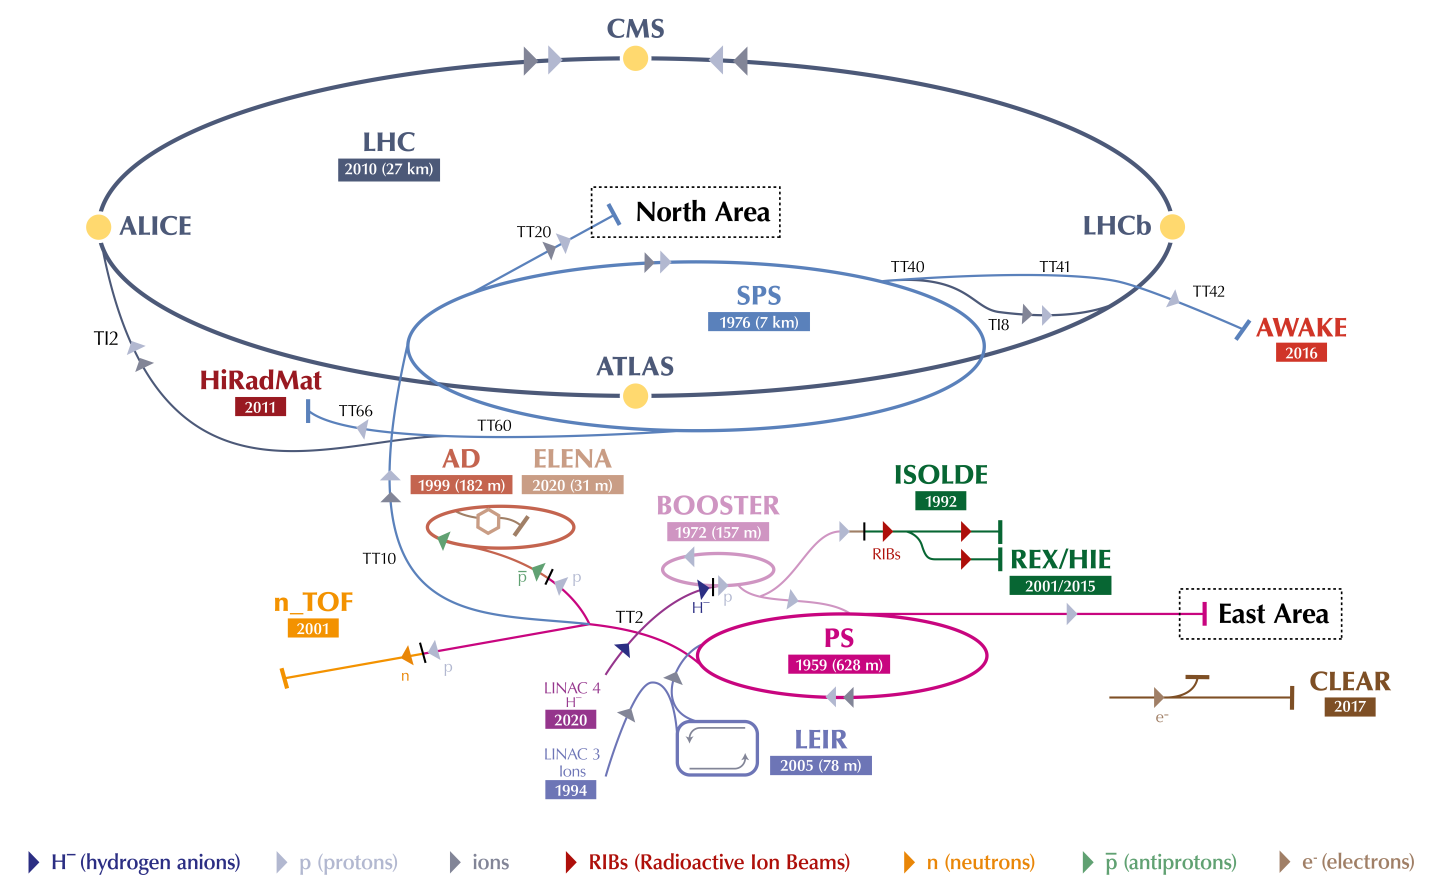
\includegraphics[width=0.8\linewidth]{figures/theoryexperiment/CCC-v2019-final-white_cut}
	\caption{The accelerator complex of the LHC, their corresponding construction years and circumferences. Individual stages are shown in different colours, the particle types they accelerate are indicated as arrows. Note that the pre-acceleators do not serve the LHC ring exclusively and the diverging paths lead to other independent experiments. Old tunnels of previous experiments serve as pre-accelerators now in the LHC injection chain. \cite{Mobs:2684277}}
	\label{fig:lhcstructure}
\end{figure}

The four main stages of pre-acceleration for protons are listed in tab. \ref{tab:preaccelerators} below. As proton source, hydrogen is used. The protons are first accelerated in the form of H$^-$ ions through the 86 metre long tunnel of the recently (2020) constructed Linear Accelerator 4 (Linac4). Stripped of their pair of electrons, the protons enter the Proton Synchrotron Booster (PSB) where they reach up to \SI{2}{\giga\electronvolt}. In the next step of the injection chain, they enter the Proton Synchrotron (PS), historically the first synchrotron at CERN serving exclusively as a pre-accelerator now. Travelling through the 628 metres long ring and accelerated to 26 GeV, the particles are injected into the Super Proton Synchrotron (SPS), where they are awaiting injection into the LHC once they reach 450 GeV.

%https://home.cern/science/accelerators/linear-accelerator-4
%https://home.cern/science/accelerators/proton-synchrotron-booster
%https://home.cern/science/accelerators/proton-synchrotron
%https://home.cern/science/accelerators/super-proton-synchrotron
%https://home.cern/science/accelerators/large-hadron-collider

\begin{table}[h!]
	\centering
	\begin{tabular}{c|c}
		Accelerator & Peak Energy \\
		\hline
		\hline
		Linear accelerator 4 (Linac4) & 160 MeV \\
		\hline
		Proton Synchrotron Booster (PSB) & 2 GeV \\
		\hline
		Proton Synchrotron (PS) & 26 GeV \\
		\hline
		Super Proton Synchrotron (SPS) & 450 GeV \\
		\hline
		Large Hadron Collider (LHC) & 7 TeV \\
	\end{tabular}
	\caption{The acceleration chain the protons undergo to reach their final energy of 7 TeV.}
	\label{tab:preaccelerators}
\end{table}

In the LHC the beams are circulating in opposing directions. They are kept on a circular trajectory using superconducting NbTi magnets operating at \SI{1.9}{\kelvin} thanks to the superfluid helium bath at about \SI{0.13}{\mega\pascal} \cite{Brüning:782076}. In the tunnel itself there are eight interactions points (IP). ATLAS, ALICE, CMS and LHCb are located at IP1, IP2, IP5 and IP8, respectively. IP3 and IP7 are where the momentum and betatron collimators are located ensuring beam quality; the radiofrequency (RF) cavities are at IP4 increasing the bunch energy to 7 TeV. The beam dump is at IP6 where old bunches are deflected by the fast-pulsing "kicker" magnets and directed towards the carbon absorber at the end of their lifetime. \cite{Evans_2008}

\begin{figure}[h!]
	\centering
	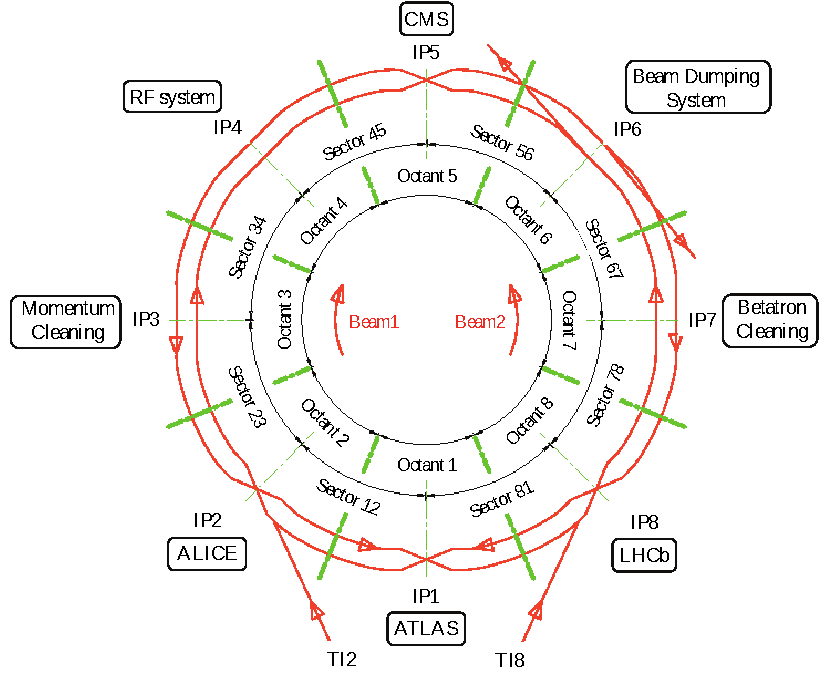
\includegraphics[width=0.6\linewidth]{figures/theoryexperiment/LHC_ring.pdf}
	\caption{The location of the interaction points, the experiments, and the beam adjustment systems. The LHC ring is also divided into further sectors and octants for each IP. \cite{Bracco:1174254}}
	\label{fig:LHC_ring}
\end{figure}

The four main detectors perform the particle collision measurements. LHCb specializes on flavour physics and measures b-quark decays focussing on the measurement and study of CP-violating processes. ALICE has been constructed to mainly study the quark-gluon plasma resulting from heavy ion collisions. ATLAS and CMS are sister experiments and are general purpose detectors. In the following, the latter will be described in detail only.

\Subsection{The Compact Muon Solenoid}

\textcolor{red}{The Compact Muon Solenoid (CMS) detector is a 14 000 tonnes heavy detector measuring .... metres and .... metres.} While it has been built to be general purpose, it features additional muon chambers at its most outer side allowing the precise measurement of muon momenta. It has several subdetector components which surround the beampipe in a layered, onion-like structure. CMS has rotational symmetry around the beampipe along which the z-axis is usually defined. The positions of each components and some of their most important technical details are shown in fig. \ref{fig:cms_view}.

\begin{figure}[h!]
	\centering
	\includegraphics[width=0.8\linewidth]{figures/theoryexperiment/cms_160312_02.pdf}
	\caption{from \cite{Sakuma:2665537}}
	\label{fig:cms_view}
\end{figure}

\begin{figure}[h!]
	\centering
	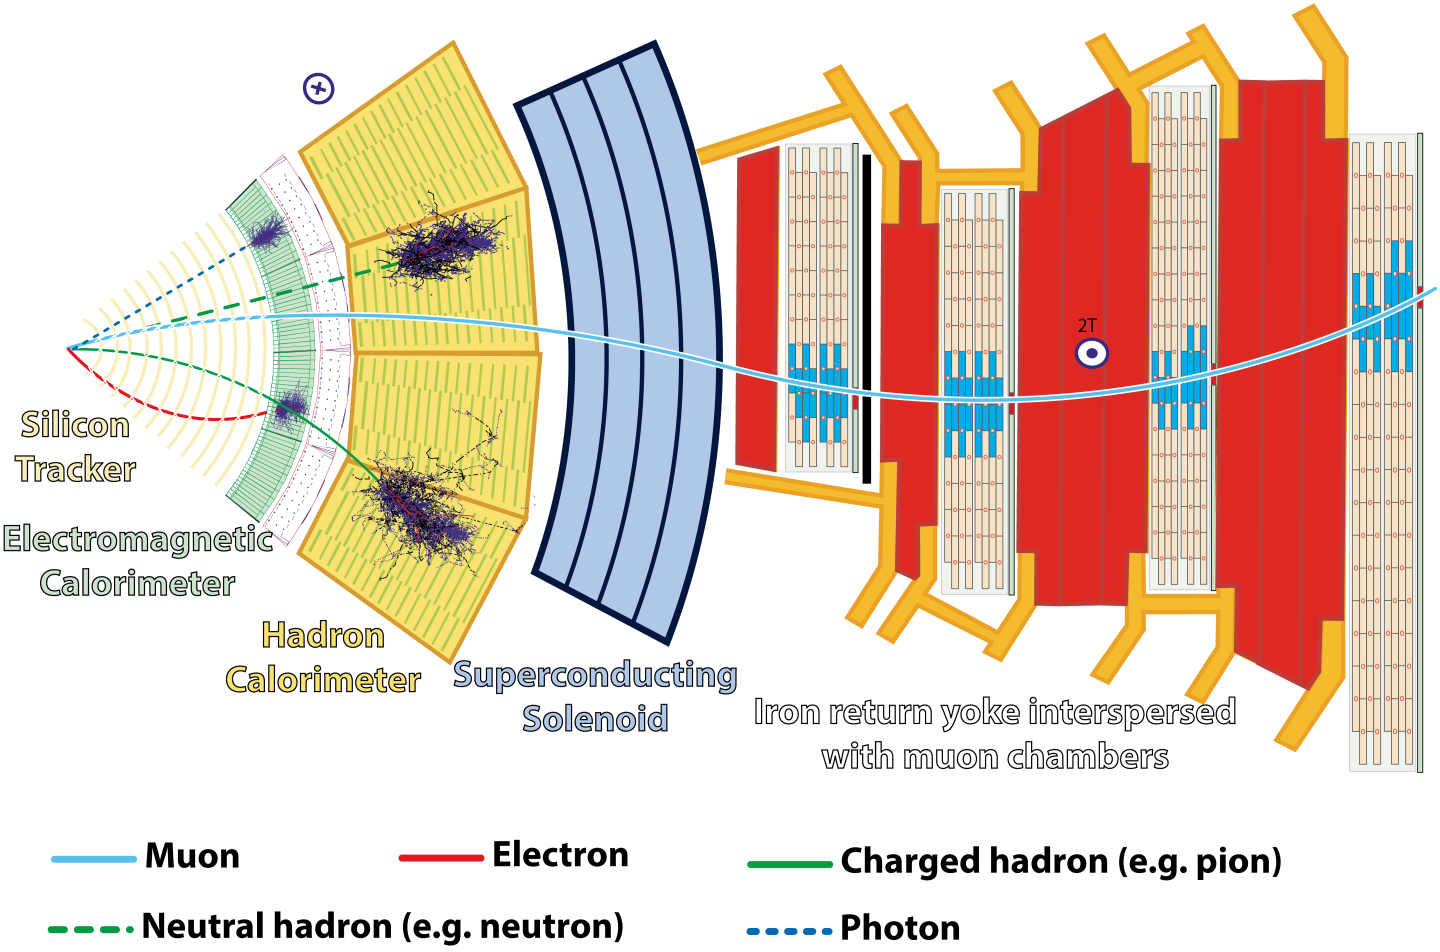
\includegraphics[width=0.8\linewidth]{figures/theoryexperiment/CMS_Slice}
	\caption{from \cite{Barney:2120661}}
	\label{fig:cms_slice}
\end{figure}
